\documentclass{article}
\usepackage[utf8]{inputenc}
\usepackage{mathtools}
\usepackage{amsmath}
\usepackage{graphicx}

\title{Gaussian Process Regression}
\author{Hafiz Hashim Imtiaz }
\date{January 2020}

\begin{document}

\maketitle

\section{Introduction}
A Gaussian process defines a distribution over functions such that, if we pick any two or more points in a function (i.e., different input-output pairs), observations of the outputs at these points follow a joint (multivariate)
Gaussian distribution. More formally, a Gaussian process is defined as a collection of random variables, any finite number of which have a joint (multivariate) Gaussian distribution. 
\\*
\\*
The Gaussian distribution or normal distribution is the foundation of Gaussian process. The uni-variate Gaussian distribution is defined by the mean $(\mu)$ and the variance $(\sigma^2)$. Similarly the multivariate Gaussian distribution is defined by a mean vector
$(\mu)$ and covariance matrix $(\Sigma)$. The mean vector depicts the expected value of the distribution. While the covariance matrix $(\Sigma)$ shows the variance along each dimension and calculates the correlation between the different random variables. 
\\*
\\*
A random vector $x = (X_1,\dots,X_N)$ is completely defined by $(\mu)$ and $(\Sigma)$, so it is convenient to write:
\\*
\\*
$$x \sim \mathcal{N}{\left(\mu, \Sigma\right)}$$
\\*
\\*
Gaussian processes allow us to invent predictions about our data by using prior knowledge. It helps us in fitting the function into the data which we also called regression. Let us suppose we have a training data, there could be several functions that could fit that data. Gaussian Process assign probability to each of these functions
\\*
\\*
A Gaussian Process defines a prior over functions which can be transformed into a posterior over functions after observing some data. It is challenging to show the distributions over functions, instead we define distributions over the values of functions at some definite arbitrary set of points. Let we have a set of points $x = (x_1,\dots,x_N)$, a Gaussian process considers that $p(f(x_1),\dots,f(x_N))$ is jointly Gaussian containing some mean and covariance matrix. 
\\*
Consider we have the joint probability of two random variables $x_1$ and $x_2$ as follows:
\\*
$$\begin{pmatrix}
x_1 \\
x_2
\end{pmatrix}
\sim \mathcal{N}{\left(
\begin{pmatrix}
\mu_1 \\
\mu_2
\end{pmatrix}
,
\begin{pmatrix}
\sigma_{11} & \sigma_{12}\\
\sigma_{21} & \sigma_{22}\\
\end{pmatrix}
\right)}$$
\\*
where $(\mu_1)$ and $(\mu_2)$ are the elements of the mean vector and $(\sigma_{11})$, $(\sigma_{12})$, $(\sigma_{21})$ and $(\sigma_{22})$ are the elements of covariance matrix. The covariance matrix is always positive-semi definite and symmetric. The diagonal elements of covariance matrix show the variances of individual random variables while the off-diagonal elements depicts the correlation between two random variables. So generally we can write:
\\*
$$\Sigma_{ij} = k(X_i,Y_j)$$
\\*
$k(X_i,Y_j)$ is the covariance of $X_i$ and $Y_j$ . Where k is a kernel or covariance function. 
\\*
The most interesting and important part of Gaussian process is to build the covariance matrix by evaluating the covariance function k pairwise on all points from the set of points. The covariance function gets two points as input and returns a scalar value which shows the similarity between two given points. The two points given to the covariance function could be from the training set or test set, depend on the element of covariance matrix we want to evaluate. The covariance matrix defines the shape of our distribution and also determines the aspects of the output function we want to predict. 

\section{Regression}
We assume a function f, the output of the function at x is y. We can write it as:
\\*
$$y = f(x)+\epsilon$$
$$\epsilon \sim \mathcal{N}{\left(0, \sigma_{\epsilon}^2\right)}$$
\\*
Where $\epsilon$ is the noise term and $f(x)$ is a signal term. The signal term is considered as a random variable which also follows an appropriate distribution. The distribution shows the uncertainty regarding the function. We reduce this uncertainty by observing the output values by giving different inputs to the function.   The noise term defines randomness in the observations. A Gaussian process is completely specified by its mean and covariance function.  In a Gaussian process regression, we considers $f(x)$ is distributed as a Gaussian process. We can write it as:
\\*
$${f(x)\sim \mathcal{GP}{\left(m(x),k(x,x')\right)}}$$
\\*
$$m(x) = E(f(x))$$
\\*
$${k(x,x')= E((f(x)-m(x)-f(x')-m(x'))}$$
\\*
The mean function $m(x)$ is actually the expected value of the function at input $x$. We set the prior mean function to zero to avoid difficult posterior calculations. We need to do assumptions based on covariance functions which figures the dependence between the function values at different input points. 
The choice of the appropriate kernel is very important in Gaussian process regression. One of the common assumption is that the correlation of two points should be decreases with the increase of distance between points. More precisely we can say that the two points which are placed closely will behave more similarly that the two points which are far away from each other. The radial basis or squared exponential covariance function shown below fulfills this assumption. 
\\*
$$k(x,x')=\sigma_f^2 \exp-(\frac{{{||(x-x')||}^2}}{(2\lambda^2)})$$
\\*
There are two hyper parameters length and signal variance which increase or decrease the priory correlation between points. 
After selecting mean and kernel functions, we can use the Gaussian Process to define a prior over functions which can be transformed into a posterior over functions after observing some data.
\\*
\subsection{Sampling functions from a Gaussian Process}
Sampling of a function from a Gaussian process is usually done by calculating the function values at chosen set of input points. We can evaluate outputs of the input points by using a multivariate Gaussian distribution with a covariance matrix. Let $X_*$ be a matrix with input point ${x_i^*}, i=1,…..n$. We first compute the covariance pairwise between all inputs using covariance function and make the covariance matrix $K(X_*,X_*)$. We will choose the usual prior mean function $m(x)=0$ for the simplification. To sample a function, we first compute the covariances between all inputs in $X_*$ and collect these in an $n x n$ matrix. 
\\*
$$K(X_*,X_*) = 
\begin{pmatrix}
k(x_1^*,x_1^*) & k(x_1^*,x_2^*) & \cdots & k(x_1^*,x_n^*) \\
k(x_2^*,x_1^*) & k(x_2^*,x_2^*) & \cdots & k(x_2^*,x_n^*) \\
\vdots  & \vdots  & \ddots & \vdots  \\
k(x_n^*,x_1^*) & k(x_n^*,x_2^*) & \cdots & k(x_n^*,x_n^*)
\end{pmatrix}$$

The values of f at $X_*$ inputs can be sampled using Gaussian process using multivariate Gaussian distribution.
$$f_{*} \sim \mathcal{N}{\left(0, K(X_*,X_*)\right)}$$
If we want to find $y_*$, we just need to add an additional sample of noise $\epsilon$. 
\\*
\subsection{Posterior predictions from a Gaussian Process}
We have chosen a training set of n observations, $D = {(x_i, y_i) | i = 1, . . . , n}$. We can also write $D = (X, y)$ where $X$ is the input vector containing all the independent input samples. While $y$ is the vector of corresponding scalar outputs i.e. the targets. Now we want to predictions for new inputs $X_*$ by drawing $f_*$ from the posterior distribution. 
Importantly Bayes’ rule let us calculate the conditional probability of one of the variables given the other by the formula
$$p(D|f) = \frac{p(f|D)p(f)}{p(D)}$$
$$ Posterior = \frac{(Likelihood)(Prior)}{Normalization}$$
\\*
According to the definition, the function values f* and previous observations y follow the joint multivariate Gaussian distribution, can be written as.
\\*
$$\begin{bmatrix}
y \\
f_{*}
\end{bmatrix}
\sim \mathcal{N}{\left(0,
\begin{bmatrix}
K(X,X)+\sigma_n^2I &  K(X,X_*)\\
K(X_*,X) & K(X_*,X_*)
\end{bmatrix}
\right)}$$
\\* 
Where $K(X,X)$ is the covariance matrix between all the observed points, $K(X,X_*)$ is the covariance matrix between the observed points and newly added points and $K(X_*,X_*)$ is the covariance matrix between the newly added input points. Moreover I is the identity matrix and sigma is the added noise level(the variance of $\epsilon$). After computing conditional distribution, we derived the important predictive equations for Gaussian process regression as shown below.
\\*
$$f_{*} | X,y,X_{*}\sim \mathcal{N}{\left(\Bar{f_{*}},cov(f_{*})\right)}$$
\\*
$$\Bar{f_{*}} = E(f_{*} | X,y,X_{*}) = K(X_*,X)[K(X,X)+\sigma_n^2I]^{-1}y$$
\\*
$$cov(f_{*})=K(X_*,X_*)-K(X_*,X)[K(X,X)+\sigma_n^2I]^{-1}K(X,X_*)$$
\\*
This clears that computing the posterior mean and covariance of a Gaussian process involves first calculating the 4 different covariance matrices above and then combining  and solving them. 
To predict $f_*$, we can simply use the calculated mean and covariance functions from the GP as shown above. 
\\*
\subsection{Optimization of hyper-parameters}
The covariance function usually contains hyper-parameters such as the length-scale $(\lambda)$,signal variance $\sigma_f$, and noise variance $\sigma_n$, which are unknown and need to be predicted from the observed data. The common method to predict or compute the hyper-parameters is by maximising the marginal likelihood. For convenience, we use $\theta$  to denote the vector of
all hyper-parameters of the model. Let given the data $D={(X; y)}$ and hyper-parameters $\theta$ such that $\theta\sim(\lambda,\sigma_f,\sigma_n)$.We will chose the parametric prior.
\\*
$${p(f|\theta))}= \mathcal{GP}{\left(f;\mu(x;\theta),K(x,x';\theta)\right)}$$
\\*
We will measure the quality of the fit to our training data $D = (X; y)$ with the marginal likelihood. The equation for log marginal likelihood is shown below. 
\\*
$$\log{p(y|X)} = -\frac{{y^T}{(K(X,X)+\sigma_n^2I)^{-1}}{y}}{2} - \frac{\log|{K(X,X)+\sigma_n^2I}|}{2} - \frac{n\log{2\pi}}{2}$$
\\*
The marginal log likelihood can be seen as a penalized fit measure,
where the first term $-\frac{{y^T}{(K(X,X)+\sigma_n^2I)^{-1}}{y}}{2}$ measures the data fit. The second term $=-\frac{\log|{K(X,X)+\sigma_n^2I}|}{2}$ is a complexity penalization term and the last one $- \frac{n\log{2\pi}}{2}$ is a normalization constant.
To find the appropriate parameters, we will maximize our log marginal likelihood function using gradient ascent. For maximizing the function, we take partial derivative with respect to a specific parameter, multiply it with a learning rate and add it to the previous value of parameter. We Keep doing this until we reach to the maximum, means where derivative is zero and there is no much difference between previous and present value of the function at the specific value of parameter. We want to find this specific value of all the hyper-meters. The notation for gradient acsent is shown below:
\\*
$$\theta_j \leftarrow \theta_j+\alpha \frac{\partial}{\partial \theta_{j}} J(\theta)$$
\\*
\section{Implementation of Gaussian Process Regression}
\subsection{Training Samples}
$$ x = [1., 2., 4., 5., 6., 8., 9., 11.]$$
$$ f(x)= xsin(x)$$
$$ y = f(x)+\epsilon$$
$\epsilon \sim \mathcal{N}{\left(0, \sigma_{n}^2\right)}$ with $\sigma_{n}=0.5$
\begin{figure}[]
    \centering
    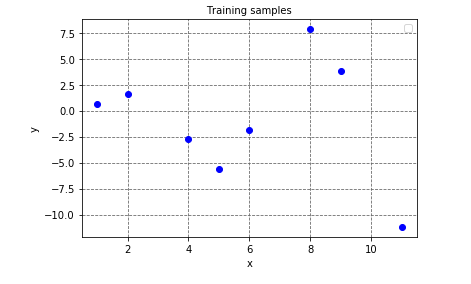
\includegraphics[width=12cm]{Capture.PNG}
    \caption{Training Samples}
    \label{fig:Training samples}
\end{figure}
\subsection{Prediction of Test Samples and Function}
$$ x_{*} = [3., 7., 12.]$$
$$x_1^* = 3$$
$$\Bar{f_1^{*}}= 0.00487715$$
$$cov(f_1^{*}) = 0.43065218$$
$$x_2^* = 7$$
$$\Bar{f_2^{*}}= 3.12862462$$
$$cov(f_2^{*}) = 0.43050401$$
$$x_3^* = 12$$
$$\Bar{f_3^{*}}= -5.71760244$$
$$cov(f_3^{*}) = 0.70278781$$
\\*
\begin{figure}[]
    \centering
    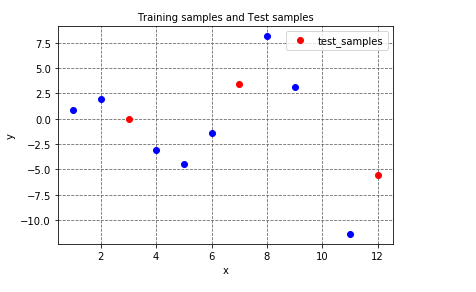
\includegraphics[width=12cm]{Capture2.PNG}
    \caption{Prediction of Test Samples with $\sigma_n = 0.5$, $\sigma_f=1$ and $\lambda=1$}
    \label{fig:Test samples}
\end{figure}
\\*
\begin{figure}[]
    \centering
    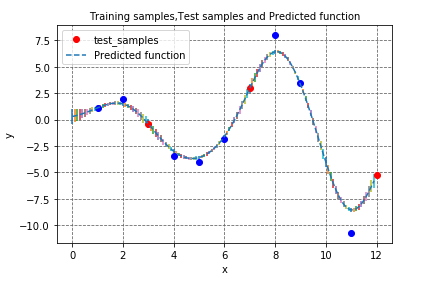
\includegraphics[width=12cm]{Capture3.PNG}
    \caption{Prediction of Function with $\sigma_n = 0.5$, $\sigma_f=1$ and $\lambda=1$}
    \label{fig:Function prediction}
\end{figure}
\\*
\begin{figure}[]
    \centering
    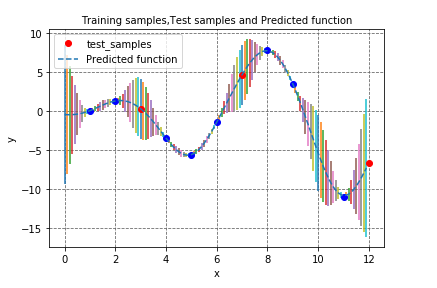
\includegraphics[width=12cm]{Capture4.PNG}
    \caption{Prediction of Function with $\sigma_n = 0.5$, $\sigma_f=4$ and $\lambda=1$}
    \label{fig:Function prediction2}
\end{figure}
\\*
After gradient ascent optimization, we have found the optimal values of $\sigma_f$ and $\lambda$. The values are
$$\sigma_f=8$$ 
$$\lambda=1.9$$
\\*
\begin{figure}[]
    \centering
    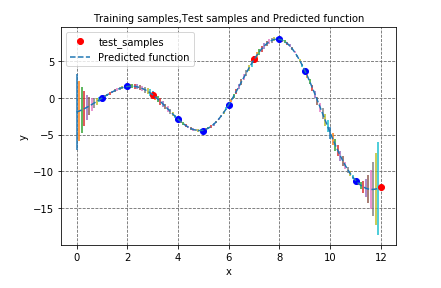
\includegraphics[width=12cm]{Capture5.PNG}
    \caption{Prediction of Function with $\sigma_n = 0.5$, $\sigma_f=8$ and $\lambda=1.9$}
    \label{fig:Function prediction3}
\end{figure}
\end{document}